%%% TEMPLATE FOR Extended Abstract Track (non-archival) %%%%
\documentclass[mlabstract,onecolumn]{jmlr}

% The following packages are loaded automatically by jmlr.cls and MUST NOT be
% re-added here (INSTRUCTIONS.txt): amsmath, amssymb, natbib, graphicx, url,
% algorithm2e.
\usepackage[T1]{fontenc}
\usepackage{booktabs}
\usepackage{bm}
\usepackage{microtype}

%%%% DON'T CHANGE %%%%%%%%%
\jmlrvolume{}
\firstpageno{1}
\editors{}

\jmlryear{2026}
\jmlrworkshop{Symmetry and Geometry in Neural Representations}
%%%%%%%%%%%%%%%%%%%%%%%%%%

\title[The Price of a Flat Direction]{The Price of a Flat Direction: Transverse Curvature sets Retention in a Trained Recurrent Memory}

% THE MANUSCRIPT, DATA AND CODE MUST BE ANONYMIZED DURING THE REVIEW PROCESS.
% Author block intentionally omitted for double-blind review.
% We evaluate a recurrent unit that advances a latent state $(q,p)$ via a damped symplectic velocity-Verlet step of a learned Hamiltonian that governs latent-space dynamics.
\begin{document}
\maketitle
\begin{abstract}
Recurrent neural networks can store continuous latent values on a marginally stable latent manifold. Prior work establishes that such a manifold is fragile: noise diffuses the state along the manifold, most infinitesimal perturbations to the dynamics destroy it, and exact equivariance protects a neutral direction with zero Lyapunov exponents tangent to the group orbit. \emph{However}, while the kinematics of symmetry protection are known, the quantitative relationship, i.e. how the retention of a written value scales with the transverse curvature of a trained latent surface, remains unmeasured. \emph{In this work, we measure this relationship} on a trained manifold. The trained latent potential $V_\theta$ is $G$-invariant with minimisers on a $G$-orbit, representing spontaneous symmetry breaking, such that the curvature $\mu$ transverse to the orbit determines the survival time of a written value within limits. As an initial empirical study, we measure this retention profile and find that the retention half-life follows $n_{1/2}\propto\mu^{-2}$. This scaling law halts at a crossover boundary $\varepsilon\mu\approx\gamma/2$, beyond which the half-life saturates at a curvature-independent floor. Furthermore, this retention profile survives the training-time correction required to maintain the orbit, where the objective naturally degrades it.
\end{abstract}

\section{Introduction}\label{sec:intro}

A latent memory register, defined as a recurrent state designed to hold an analog value, can be built on a flat direction: a continuous set of states that the network dynamics do not distinguish, ensuring a written value neither decays nor converges to a preferred attractor. Symmetries supply these directions natively through spontaneous symmetry breaking~\citep{iqbal_spontaneous_2026}. \emph{However}, while the theoretical existence of such a flat direction is established~\citep{golubitsky_singularities_1988,krupa_bifurcations_1990,rumberger_lyapunov_2001,mo_symmetry-protected_2026}, its operational utility as an AI memory mechanism depends on a non-exhaustive, quantitative checklist: how much retention is gained for a given transverse curvature, the boundaries of this scaling law, and the stability of the manifold against corrective training mechanisms. \emph{Therefore, we explicitly measure these three properties on trained models.}

\paragraph{Contributions:} We structure our contributions as follows:
\begin{enumerate}
\item \emph{The curvature-retention relationship (CRR)} (Sec.~\ref{sec:pricelist}, Sec.~\ref{sec:cure}): We establish this relationship, identify the crossover boundary where this law halts, and demonstrate its survival under training-time corrections that preserve the orbit.
\item \emph{Evidence on a learned system} (Sec.~\ref{sec:headtohead}): We evaluate a recent single-exponential lifetime estimator~\citep{mo_symmetry-protected_2026} directly on our trained checkpoints. It aligns with our CRR in the overdamped regime but predictably fails above the crossover boundary.
\item \emph{Operational boundaries and negative results} (Sec.~\ref{sec:boundary}): We explicitly outline the limits of our findings. On this architecture class, flat directions must be designed rather than trained for; the continuous register poorly transfers to an emergent potential; and the retention efficiency relative to recurrent baselines inverts when normalized for compute.
\end{enumerate}

This work does not propose a new architecture, but rather provides a closed-form analysis of latent retention on a trained recurrent model~\citet{jawahar_chlu_2026}. The laws are derived for the class of damped symplectic recurrences; we verify them on one trained instance. See App.~\ref{app:defs} for definitions of terminology used in our scope.

\section{Related work and positioning}\label{sec:related}

The intersection of temporal deep learning dynamics and symmetry-driven learning frameworks converges on the continuous attractor on a manifold~\citep{golubitsky_singularities_1988,krupa_bifurcations_1990,rumberger_lyapunov_2001, sagodi_back_2025, seung_how_1996}.

The literature also establishes fundamental constraints on continuous attractors. Noise drives diffusion along the manifold, lower-bounded by the code's Fisher information~\citep{burak_fundamental_2012}. Furthermore, these manifolds are structurally unstable and generally destroyed by infinitesimal perturbations to the dynamical rules, an issue termed the \emph{fine-tuning problem} in online learning~\citep{sagodi_back_2025}. Homeostatic mechanisms to restore these flat directions are well-documented~\citep{renart_robust_2003}, and local learning rules have been shown to produce accurate ring-attractor tuning~\citep{vafidis_learning_2022}. Approximate continuous attractors also emerge analytically during task training~\citep{dinc_ghost_2026}. \emph{However}, the literature currently lacks a precise relationship linking transverse curvature to retention capacity of trained models, including the crossover bounds of such laws. \emph{We address this gap}. Further related works motivating this paper are presented in App.~\ref{app:relpos}.

\section{Setup}\label{sec:setup}
\paragraph{Dynamical mapping and retention bands:} One dissipative velocity-Verlet step (defined by step $\varepsilon$ and damping $\gamma$) advances the latent state $(q,p)$ via a kick-drift-kick of the Hamiltonian $H=T(p)+V_\theta(q)$, followed by the damping map $p\mapsto(1-\gamma)p$; presented here as the Causal Learning Unit (CLU). As in prior works like the CHLU, the Hamiltonian dynamics only define how the latent state evolves, parametrized by some encoder and is unrelated to the input space without it. This map is conformally symplectic, satisfying $J^\top\Omega J=(1-\gamma)\Omega$ and $\det J=(1-\gamma)^d$, where $d$ is the dimensionality of the latent $q$ or $p$. Phase-space volume subsequently contracts by a fixed factor at each step, preserving geometry while diminishing scale. The memory dynamics at each normal mode reduce to a $2\times2$ block defined by $\mu^2=k/m$ and the leapfrog stability parameter $h=\varepsilon\mu$~\citep{hairer_geometric_2006}. The retention behavior splits into three explicit bands:
\begin{itemize}
    \item \textbf{The Latch:} ($\mu=0$, symmetry-protected). Exhibits frozen displacement $q_\infty=q_0+\varepsilon p_0/(M\gamma)$ and an infinite half-life.
    \item \textbf{The Overdamped Register:} ($0<\varepsilon\mu\lesssim\gamma/2$). Resolves to a half-life of $n_{1/2}\approx2\gamma\ln2/[(2-\gamma)(\varepsilon\mu)^2]$.
    \item \textbf{The Underdamped Working Memory:} ($\gamma/2\lesssim\varepsilon\mu<2$). Bound by a curvature-independent envelope half-life of $2\ln2/(-\ln(1-\gamma))$.
\end{itemize}
The boundary separating the overdamped and underdamped regimes is the exceptional point $h^*\approx\gamma/2$, where the block matrix becomes defective (derived in App.~\ref{app:derivation}). For further map definition, the curvature instantiation and coset storage details see App.~\ref{app:curcos}.

\section{Results: the CR relationship, its evidence, and its boundary}\label{sec:results}

\subsection{Effects of latent manifold curvature, and where the law stops}\label{sec:pricelist}

While a zero eigenvalue formally certifies that a direction is neutral, it does not quantify the retention cost of a near-zero curvature. \emph{Therefore, we apply a controlled analytic tilt to a trained potential, measure the resultant transverse curvature via its Hessian, and evaluate the retention half-life of the stored value.}

On the trained designed vacuum, the flat mode measures at $\mu^2\le2.4\!\times\!10^{-15}$ (machine precision). The constitutive identity holds robustly: the Hessian-derived spectral mass aligns with the measured one-step-Jacobian gap to $3.2\!\times\!10^{-10}$ across all $70$ tilt configurations. Consequently, the retention law follows precisely, with a curvature ratio $\mu^2_{\mathrm{meas}}/\mu^2_{\mathrm{pred}}=1.000000\pm5\!\times\!10^{-12}$ at every tilt and seed across $4.5$ orders of magnitude. The fitted overdamped slope is $-0.985$ ($n=35$) as shown in Fig.\ref{fig:pricelist}, closely matching the theoretical $-1$. Beyond the crossover boundary, the half-life decouples from curvature entirely, saturating at a floor of $27.03$ steps for $\gamma=0.05$. See App.\ref{app:resEx} for further results on this. These results utilize analytic tilts on trained checkpoints, serving as exact verification of the theory rather than emergent discoveries (further detailed in Appendix~\ref{app:gmor}).


\begin{figure}[htbp]\centering
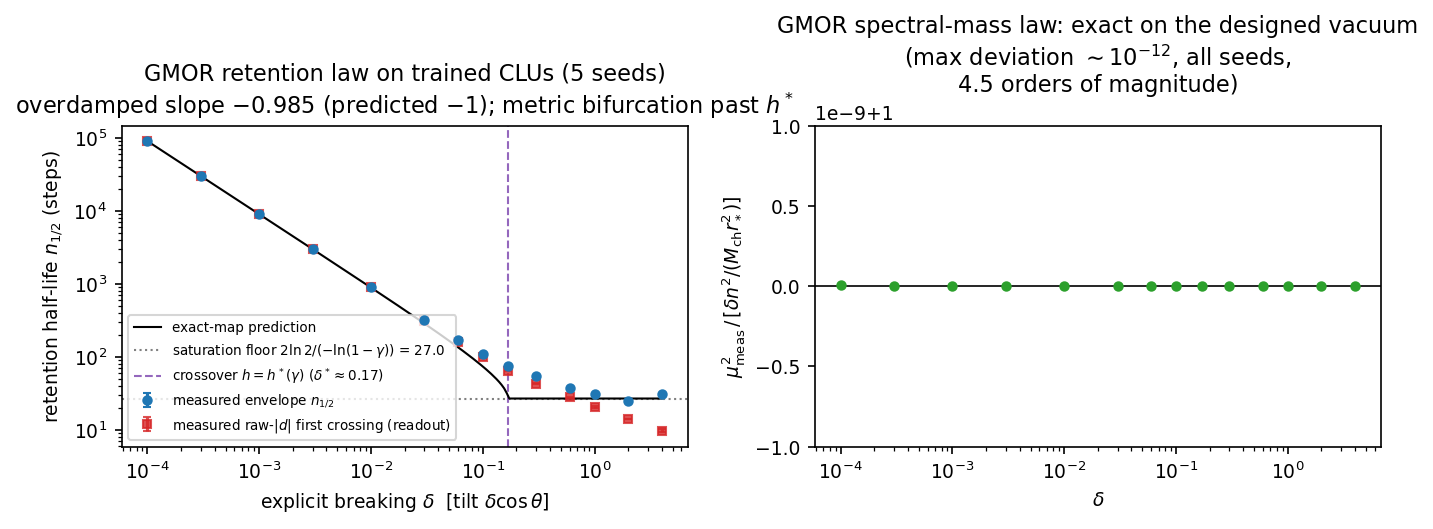
\includegraphics[width=0.85\linewidth]{figs/fig1_gmor.png}
\caption{The curvature-retention relationship, verified on trained checkpoints. Left: The retention half-life $n_{1/2}$ against the analytic tilt $\delta$. The overdamped branch tracks the predicted law at a fitted slope of $-0.985$ (predicted $-1$) before saturating past $h=h^*(\gamma)$ at the curvature-independent floor of $27.03$ steps ($\gamma=0.05$). Envelope half-life (circles) and raw first-crossing time (squares) diverge after the crossover exceptional point. Right: The curvature identity holds flat at $1.000000\pm5\times10^{-12}$ across $4.5$ orders of magnitudes of $\delta$. \emph{Setup: Trained designed checkpoints, analytic tilts, $5$ seeds, dim $4$, $\gamma=0.05$.}(Figure downsized for space constraints, see App.\ref{app:resEx})}
\label{fig:pricelist}
\end{figure}

\subsection{Evidence: The lifetime estimator in~\citet{mo_symmetry-protected_2026} is the CRR's overdamped face}\label{sec:headtohead}

An established retention model should accurately predict independent metrics of decay. \emph{To evaluate this, we apply a recently posted lifetime estimator unchanged onto our trained models.}

The single-exponential estimator presented in~\cite{mo_symmetry-protected_2026} isolates a finite memory lifetime using a single-exponential estimator driven by a Lyapunov exponent (inverse time). Our formulation utilizes potential curvature (inverse time squared). We map these directly by executing their exact code-level protocol (phase $0.35$ rad, threshold $0.2$ rad, censoring cap $15000$ steps) over our approach across $5$ seeds and $14$ breaking magnitudes. In the overdamped regime, the measured-to-predicted ratio ranges from $1.012\pm0.000$ to $1.029\pm0.001$, closely matching their reported median of $1.013$.

\emph{However}, this estimator functions exclusively as the overdamped face of our framework ($\mathrm{corr}(\log\mathrm{pred},\log\mathrm{meas})=0.9987$, overdamped-only). The estimator fails predictably above the exceptional point crossover, mispredicting by $\approx3.2\times$ at the deepest trained-model breaking magnitude ($\delta=4$), exhibiting a $2.202\pm0.155$ delay spike at the crossover, and declining to $0.309\pm0.012$ deep in the underdamped regime. On exact analytic maps, this divergence extends to $\approx5\times$. This represents theoretical containment rather than conflict: our framework recovers their findings below $h^*$ and correctly models the regime structure (floor, ringing, exceptional point) above it, which standard first-order dynamical systems inherently miss.

\begin{figure}[htbp]\centering
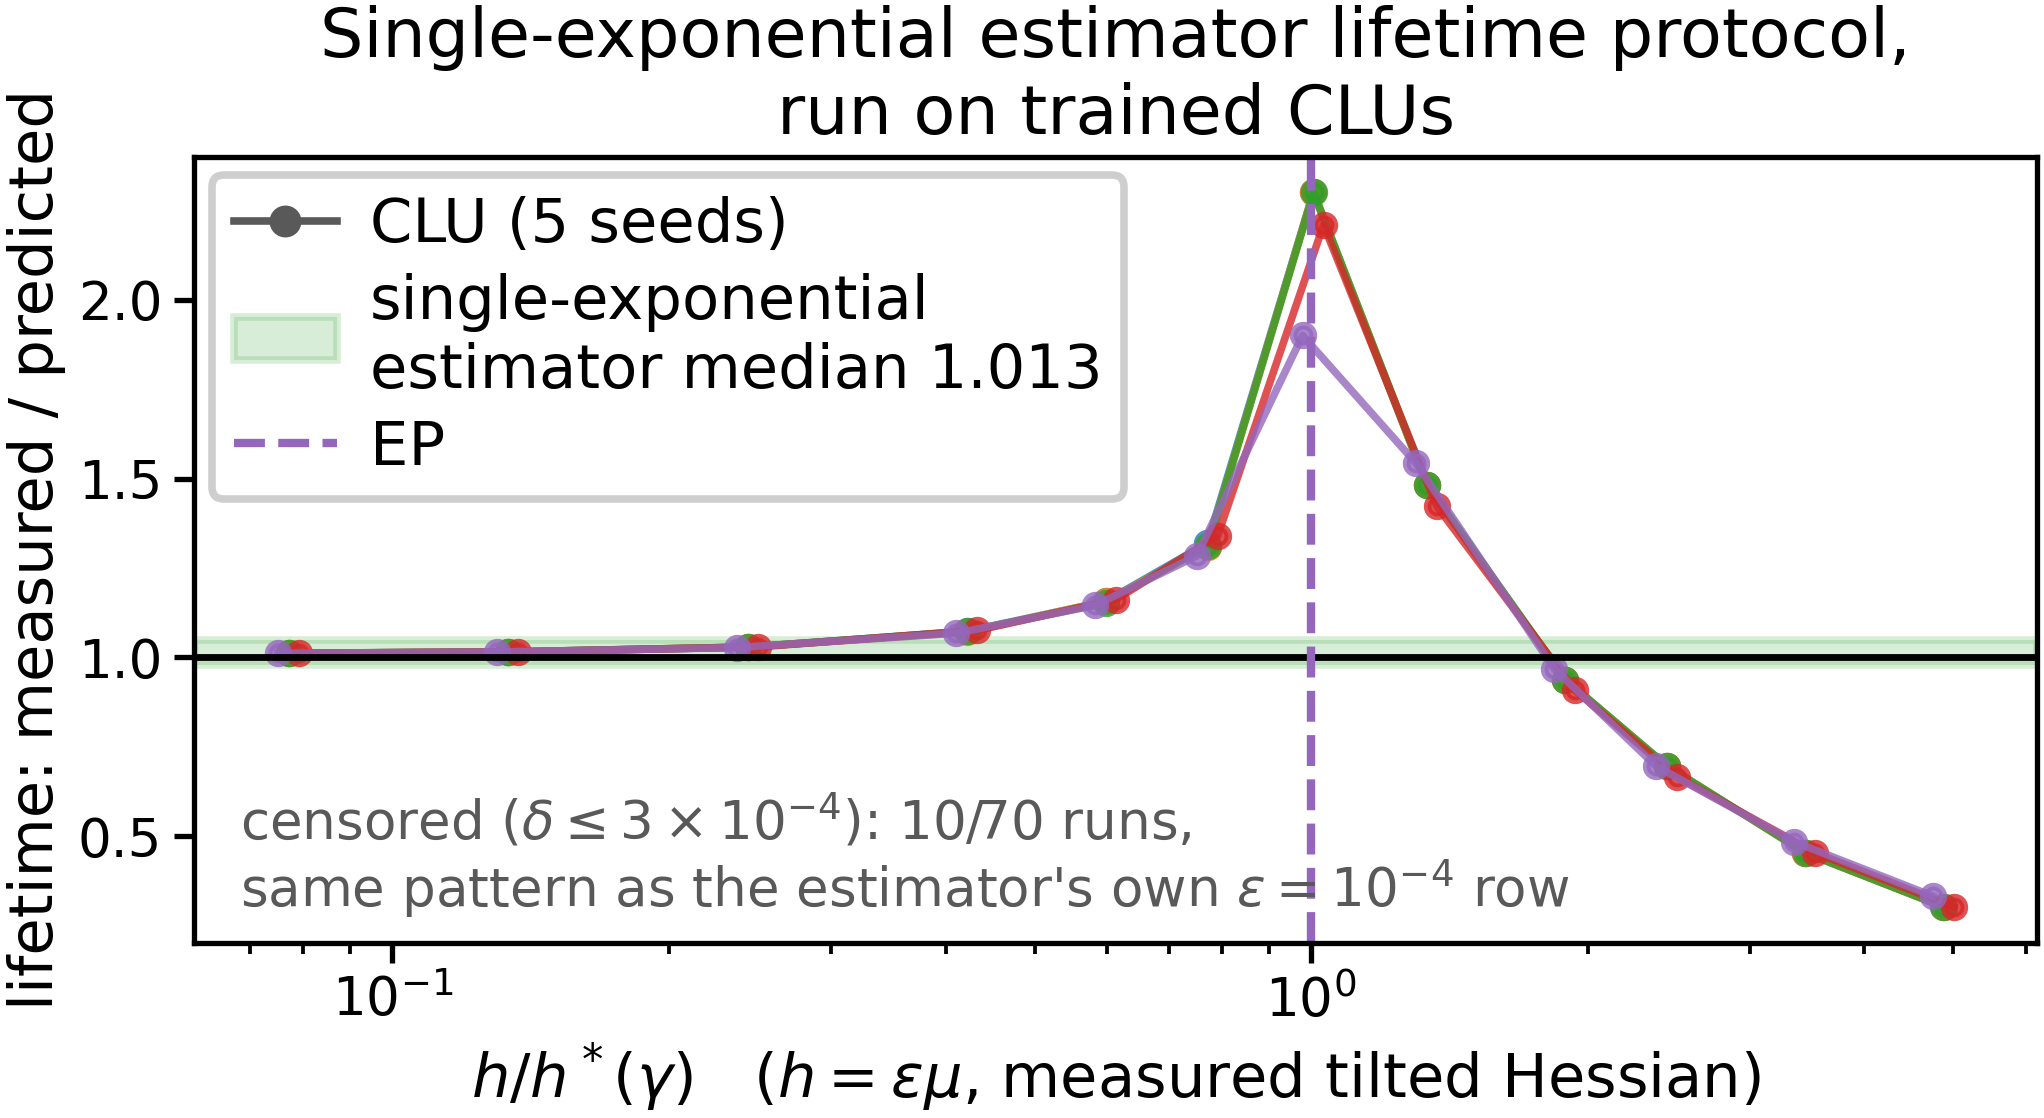
\includegraphics[width=0.33\linewidth]{figs/fig_lifetime_headtohead.png}
\caption{The single-exponential lifetime estimator from~\citet{mo_symmetry-protected_2026}, run unchanged on trained checkpoints, acts as the overdamped face of the CRR. The ratio of measured to predicted lifetime versus breaking magnitude shows containment ($\approx1$) in the overdamped regime. It exhibits a $2.2\times$ delay spike at the exceptional point and degrades to $0.31\times$ underdamped, validating the bounded limits of first-order single-exponential estimation. (Figure downsized for space constraints, see App.\ref{app:resEx})}
\label{fig:lifetime_headtohead}
\end{figure}

For results on the CRR surviving training-time corrections and for results on where the CRR does not extend, see App.~\ref{app:resEx}.

\paragraph{Autonomous retention against learned baselines:} Gated and oscillatory recurrent networks reliably minimize task error. \emph{However, fitting the task does not equate to holding a continuous latent state autonomously.} We write a latent phase into optimized baseline models (LSTM, LEM, and coRNN trained with learning rate sweeps) and allow them to run autonomously without input. The structural triad: the exact latch, the $\mu^{-2}$ scaling law, and the bounded coordinate motion, is completely absent in these baselines. Under autonomous execution, coRNN, LEM, and LSTM lose the stored analog phase within $\approx5.6/56/69$ map-steps, respectively, with coordinates randomizing beyond $1.2$ rad. In contrast, the generically-trained CLU holds for $\approx263$ map-steps with strictly bounded coordinate motion ($\approx0.35$ rad). Crucially, the designed unit never drifts across all $5$ seeds as expected. We present this result with the added caveat that the current results are empirical evidence only, generated by a local Apple M1 chip. Extensive results on real data are the next steps for our work. We also acknowledge that the compute efficiency of the CLU is much worse (see App.\ref{app:compute}) than the baselines; however, being an early-stage idea we defer compute optimization to future work when the algorithm reaches desired maturiity.

\section{Discussion}\label{sec:discussion}

By quantifying the CRR, we shift the operational perspective on flat directions. A trained memory network is best interpreted as a composite of exact latches (symmetry-protected moduli of $V_\theta$) and tunable registers (nearly-flat modes bounded by $\mu^2$). Kinetic isotropy acts as the price for an equivariant write current, rather than the register itself. Promising future directions include measuring the $\mu^{-2}$ crossover and floor at latent dimensions $\gtrsim64$ (where mode mixing may complicate the reduction), analyzing solution degeneracy between the designed and emergent arms~\citep{huang_measuring_2025}, integrating equivariant-control wrappers for supervised tasks, and generalizing the CRR beyond abelian $SO(2)$ to higher-dimensional tori and non-abelian groups. See App.\ref{app:exDisc} for further thoughts.

\bibliography{refs}

\appendix

\section{Extended Setup and Definitions}
\label{app:defs}
We analyze an architecture that advances a phase-space state $(q,p)$ through a symplectic velocity-Verlet step using a learnable separable Hamiltonian $H(q,p)=T(p)+V_\theta(q)$ similar to~\citet{jawahar_chlu_2026}, presented here as the Causal Learning Unit (CLU), to allow future generalization beyond Hamiltonian formulations of the latent dynamics. A per-step damping map $p\mapsto(1-\gamma)p$ is applied to supply controllable forgetting.

\paragraph{Definitions and conversions:} To understand the motivation for this work better, we start with a short primer on the two distinct ``mass'' quantities (that are parameters of latent dynamics and not the input space) utilized, which operate in inverse alignment.
\begin{itemize}
    \item \textbf{Inertial mass ($M_i$):} The learned diagonal entries of the kinetic term $T$. A larger $M_i$ yields slower dynamics.
    \item \textbf{Spectral mass ($\mu_k$):} The \emph{transverse curvature}, where $\mu_k^2=\lambda_k(M^{-1/2}\nabla^2V_\theta M^{-1/2})$ at a critical point. A larger $\mu$ results in shorter memory retention.
\end{itemize}
All retention laws in this paper are formulated using $\mu$. Crucially, we avoid arbitrary unit rescaling between inverse time (flow-Jacobian eigenvalues or Lyapunov exponents) and inverse time squared ($\mu^2$, eigenvalues of a mass-whitened potential Hessian). Instead, cross-field comparisons (Sec.~\ref{sec:headtohead}) are performed strictly by running published rate-based estimators unchanged on our trained models. Furthermore, what the broader literature refers to as \emph{memory lifetime} is standardized here as the half-life $n_{1/2}$, measured in map applications. Metrics such as time constants ($\tau$) or diffusion coefficients ($D$) are evaluated and reported explicitly alongside the condition that defines them, as these metrics bifurcate past critical crossover thresholds.

\section{Derivation of the band structure and closed forms}\label{app:derivation}
All closed forms quoted in Sec.~\ref{sec:setup} follow from the one-step map restricted to a single mass-whitened normal mode of transverse curvature $\mu^2$ at a critical point of $V_\theta$. With $h=\varepsilon\mu$, the kick--drift--kick step followed by $p\mapsto(1-\gamma)p$ is the linear map $(q,p)^\top\mapsto A\,(q,p)^\top$ with
\begin{equation}\label{eq:block}
A=\begin{pmatrix}1-\frac{h^2}{2} & \varepsilon\\[2pt] -(1-\gamma)\,\varepsilon\mu^2\bigl(1-\frac{h^2}{4}\bigr) & (1-\gamma)\bigl(1-\frac{h^2}{2}\bigr)\end{pmatrix},
\end{equation}
so $\det A=1-\gamma$ (the per-mode statement of conformal symplecticity) and $\operatorname{tr}A=(2-\gamma)\bigl(1-\frac{h^2}{2}\bigr)$. The eigenvalues solve $\lambda^2-(\operatorname{tr}A)\,\lambda+\det A=0$:
\begin{equation}\label{eq:eigs}
\lambda_\pm=\tfrac12\Bigl[(2-\gamma)\Bigl(1-\frac{h^2}{2}\Bigr)\pm\sqrt{\Delta}\,\Bigr],
\qquad
\Delta=(2-\gamma)^2\Bigl(1-\frac{h^2}{2}\Bigr)^2-4(1-\gamma).
\end{equation}
\emph{Bands and stability limit.} $\Delta$ vanishes where $1-h^2/2=\pm\,2\sqrt{1-\gamma}/(2-\gamma)$; since $2-\gamma\mp2\sqrt{1-\gamma}=(1\mp\sqrt{1-\gamma})^2$, the two roots are
\begin{equation}\label{eq:hstar}
h^*=\sqrt{\tfrac{2}{2-\gamma}}\,\bigl(1-\sqrt{1-\gamma}\bigr)=\frac{\gamma}{2}+O(\gamma^2),
\qquad
h_{\mathrm f}=\sqrt{\tfrac{2}{2-\gamma}}\,\bigl(1+\sqrt{1-\gamma}\bigr)=2-O(\gamma^2),
\end{equation}
so $\Delta>0$ (two real eigenvalues in $(0,1)$; overdamped) for $0<h<h^*$ and $\Delta<0$ (a complex-conjugate pair; underdamped) for $h^*<h<h_{\mathrm f}$. Equation~\eqref{eq:hstar} is the crossover $h^*\approx\gamma/2$ of Sec.~\ref{sec:setup} and, read as a condition on $\gamma$ at fixed $\mu$, the critical damping $\gamma^*\approx2\varepsilon\mu$ of App.~\ref{app:gmor}. An eigenvalue reaches $-1$ iff $1+\operatorname{tr}A+\det A=0$, i.e.\ $1-h^2/2=-1$: the map loses stability at $h=2$ exactly, for every $\gamma$. At $\mu=0$ (restoring the mode mass $M$, drift entry $\varepsilon/M$), $A$ is upper triangular with eigenvalues $\{1,\,1-\gamma\}$; then $p_n=(1-\gamma)^n p_0$ and $q_\infty=q_0+(\varepsilon p_0/M)\sum_{n\ge0}(1-\gamma)^n=q_0+\varepsilon p_0/(M\gamma)$, the frozen displacement of the latch in Sec.~\ref{sec:setup}, whose unit eigenvalue gives the infinite half-life.

\emph{Exceptional point.} At $h=h^*$, $\Delta=0$ and $\lambda_+=\lambda_-=\tfrac12\operatorname{tr}A=\sqrt{1-\gamma}$. A $2\times2$ matrix with a doubly degenerate eigenvalue is diagonalisable only if $A=\lambda I$; here $A_{12}=\varepsilon\neq0$, so $A$ carries a single eigenvector and is defective (one Jordan block), with secular transients $\propto n\lambda^n$. Just above threshold, $\Delta\simeq-4(2-\gamma)\sqrt{1-\gamma}\,h^*(h-h^*)$, so the eigenvalue phase opens as $\varphi=\arg\lambda_+\propto\sqrt{h-h^*}$, the square-root onset (exponent $1/2$) measured in App.~\ref{app:resEx}.

\emph{Overdamped half-life.} For $0<h<h^*$ write the slow root as $\lambda_+=1-\delta$ and expand the characteristic polynomial to first order in $\delta$ and $h^2$: the constant terms cancel, $1-(2-\gamma)+(1-\gamma)=0$, leaving $-\gamma\delta+(2-\gamma)h^2/2=0$. Hence
\begin{equation}\label{eq:overdamped}
\lambda_+=1-\frac{(2-\gamma)h^2}{2\gamma}+O\!\bigl(h^4/\gamma^3\bigr),
\qquad
n_{1/2}=\frac{\ln2}{-\ln\lambda_+}\approx\frac{2\gamma\ln2}{(2-\gamma)(\varepsilon\mu)^2},
\end{equation}
i.e.\ $n_{1/2}\propto\mu^{-2}$: slope $-1$ in $\log n_{1/2}$ against $\log\mu^2$ (equivalently against the tilt $\delta$, since $\mu^2\propto\delta$; App.~\ref{app:gmor}).

\emph{Curvature-independent floor.} For $h^*<h<h_{\mathrm f}$ the eigenvalues form a complex-conjugate pair, so $|\lambda_\pm|^2=\lambda_+\lambda_-=\det A=1-\gamma$ regardless of $\mu$: curvature moves only the phase $\arg\lambda_\pm$, while the modulus is pinned by the determinant. The envelope contracts by $\sqrt{1-\gamma}$ per step, so $(1-\gamma)^{n/2}=\tfrac12$ gives $n_{1/2}=2\ln2/(-\ln(1-\gamma))$, the saturation floor of Sec.~\ref{sec:pricelist} ($27.03$ steps at $\gamma=0.05$).

\emph{Coset diffusion.} On the flat direction at $T>0$, with the FDT noise of App.~\ref{app:opass} written for the coset mode of inertia $F^2$ (so $\sigma^{\star2}=F^2T\gamma(2-\gamma)$), the momentum is the AR(1) sequence $p_{n+1}=(1-\gamma)p_n+\sigma^\star\xi_n$ with stationary variance $F^2T$ (equipartition) and autocorrelation $(1-\gamma)^{|k|}$, while the coordinate accumulates $\theta_N=\theta_0+(\varepsilon/F^2)\sum_{n<N}p_n$. Summing the autocovariances, $\operatorname{Var}(\theta_N)\to N\,(\varepsilon/F^2)^2\,F^2T\,(2-\gamma)/\gamma$; with $t=N\varepsilon$ and $\operatorname{Var}(\theta)=2D_\theta t$, this is $D_\theta=\varepsilon T(2-\gamma)/(2F^2\gamma)$, the coefficient quoted in App.~\ref{app:opass}.

\section{Curvature instantiation and coset storage}\label{app:curcos}
In our CLU map, relaxation onto the orbit dictates the fast normal flow, while retention governs the slow tangent flow. Unlike standard neural integrators that store values by removing damping, our flat mode requires $\gamma>0$ to prevent infinite drift, effectively forming an exact latch.

We constrain this framework to critical points of $V_\theta$, where the transverse curvature realizes one of three states on our trained models. If a learned potential $V_\theta$ is $G$-invariant but its minimiser is not, the minimisers form a $G$-orbit where the Hessian annihilates every orbit tangent, leaving the orbit coordinate neutral. This neutral coordinate acts as the Nambu-Goldstone mode~\citep{watanabe_counting_2020,minami_spontaneous_2018} of the trained potential and functions as the continuous register. \emph{First}, $\mu^2$ is exactly zero along $\dim(G/\mathcal H)$ directions when the trained minimisers form a $G$-orbit, indicating spontaneous symmetry breaking (the designed Nambu-Goldstone mode). \emph{Second}, $\mu^2$ is small but positive when an explicit algorithmic tilt breaks the orbit, creating a pseudo-Goldstone slow manifold (instantiated via analytic tilts in Appendix~\ref{app:gmor} and generic MLPs). \emph{Third}, $\mu^2$ is strictly positive when the minimiser is invariant, eliminating the orbit entirely (observed in the eroded vacuum of Sec.~\ref{sec:cure}). We rely strictly on the classical, tree-level Goldstone theorem evaluated over a Hessian. The architecture stores the \emph{coset coordinate} $q$ along the flat direction. The parameters $(\varepsilon,\gamma,T)$ map specific $\mu^2$ values to exact retention lifetimes via the three bands. Operational assumptions and scopes are further defined in App.~\ref{app:opass}.

\section{Extended related work and positioning statement}
\label{app:relpos}
The intersection of temporal deep learning dynamics and symmetry-driven learning frameworks converges on the continuous attractor on a manifold. Neutrality along group-orbit directions is a foundational principle~\citep{golubitsky_singularities_1988,krupa_bifurcations_1990,rumberger_lyapunov_2001}. This structure operates as a manifold where tangent directions are marginally stable and normal directions are strictly stable~\citep{sagodi_back_2025}. It serves as the theoretical substrate for neural integrators~\citep{seung_how_1996}.

\paragraph{Delineation from current literature:} Recent work on \emph{flow equivariance}~\citep{keller_flow_2025} extends one-parameter Lie-group symmetries through time within recurrent states to maintain long-horizon coherence in world models~\citep{lillemark_flow_2026}. We explicitly note that ``flow'' refers to a one-parameter Lie subgroup acting through time, rather than Ricci or normalizing flows. While we study the same object, continuous symmetry in a recurrent state, our focus differs. Flow-equivariant models target velocity extrapolation; we isolate the retention cost of transverse curvature without making generalization claims. Similarly, concurrent workshop work has explored soft symmetry regularization for continuous attractors. In contrast, our designed framework builds the symmetry by construction, while our emergent models utilize no symmetry regularizers, informing our boundaries in Sec.~\ref{sec:boundary}. Finally, regarding training dynamics, literature shows that temporal-consistency regularizers shape attractor geometry~\citep{haputhanthri_understanding_2025}. We analyze the inverse dynamic in Sec.~\ref{sec:cure}: our primary objective erodes a designed flat direction, necessitating an anchor to preserve it.

\paragraph{Protection mechanisms and Lyapunov spectra:} A recent preprint (arXiv:2605.03338) theoretically proves that a $C^1$ field exactly equivariant under a Lie group guarantees at least $\dim(G/\mathcal H)$ zero Lyapunov exponents tangent to the orbit. It further demonstrates that controlled symmetry breaking yields a finite memory lifetime on an $S^1$ path integration task. We do not claim novelty over these qualitative lifetime predictions or existence proofs. Instead, we contribute the exact exchange rate mapped onto a trained potential. The currencies are fundamentally distinct: Lyapunov exponents provide inverse time (kinematics), whereas our $\mu^2$ provides the transverse curvature of a potential, scaling as inverse time squared (constitutive dynamics). Lyapunov spectra evaluate vector transport but do not capture the specific latching or noise accumulation mechanics required for functional memory. We explicitly adopt the breaking-and-censoring protocol from arXiv:2605.03338 in Sec.~\ref{sec:headtohead} to run their estimator unchanged on our models.

Prior work by \citet{xu_conformal_2022} maps Lie-group representations into recurrent grid-cell networks, enforcing a torus topology over a continuous attractor. We share this geometry but introduce a precise relationship for temporal retention. Related studies optimize attractor state packing~\citep{vastola_optimal_2025} and approach memory modification through geometry~\citep{donmez_discovering_2024}. Furthermore, our designed-versus-emergent analysis mirrors the exact-equivariance-versus-symmetry-breaking dichotomy~\citep{vanderouderaa_sparse_2023,iqbal_spontaneous_2026}. Utilizing level sets to analyze tuning landscapes is established~\citep{akhtiamov_connectedness_2023,wang_level_2022}, as is leveraging canonical quotient coordinates~\citep{aslan_group_2022} and engineering equivariant memories~\citep{bernardo_shaping_2025}. We separate our work from cross-session representational drift~\citep{driscoll_dynamic_2017,aitken_geometry_2022,jude_capturing_2023}, focusing entirely on coset coordinate motion governed by our explicit dynamics. Standard baselines include LSTM~\citep{hochreiter_long_1997}, LEM~\citep{rusch_long_2022}, and coRNN~\citep{rusch_coupled_2021}, supported by conformal symplecticity principles~\citep{mclachlan_conformal_2001} and wake-sleep contrastive divergence~\citep{hinton_wake-sleep_1995,tieleman_training_2008}, which classically distorts energy landscapes~\citep{fischer_empirical_2010,nijkamp_anatomy_2020}.

\paragraph{Positioning boundaries:} To define our contributions, the following claims are defined to be out of scope (detailed fully in Appendix~\ref{app:pos}). \emph{(1)} Attention and state-space models possess retention-guarantee analogues (e.g., HiPPO-LegS, \citealp{gu_hippo_2020,jelassi_repeat_2024}). \emph{(2)} Framing retrieval as a rollout rather than a weighted sum is established by \citet{kong_reservoir-computing_2024}. \emph{(3)} Continuous dynamics do not bypass the soft-memory lineage of NTMs and DNCs~\citep{graves_neural_2014,graves_hybrid_2016,csords_improving_2019}. \emph{(4)} This framework is not positioned as a competitor to transformer architectures. Our specific contribution remains a physics-structured associative memory where retention is governed as a designed, per-item property controlled by $\mu^2$. The closest parallel architecture is Titans~\citep{behrouz_titans_2024}, which utilizes discretized damped second-order dynamics for associative memory~\citep{karuvally_exponential_2025,ramsauer_hopfield_2020}. We differ by reading out and pricing the damping and inertia natively, rather than treating them as optimizer hyperparameters.

\section{Operational assumptions, conditions and scopes}
\label{app:opass}
In this early-stage work, results derived from designed testbeds (e.g., invariant potentials, analytic tilts, spurions) serve as verification of the theory. Conversely, outcomes from learned-system, training-dynamics, and comparative baseline experiments are presented as empirical evidence. All models evaluated utilize the Experiment-D configuration of the reference unit: dimension $4$, hidden size $64$, learned-Newtonian kinetic term, $\mathrm{dt}=0.05$, a unit circle at $256$ points, and $150$ epochs (justification for avoiding $1000$ epochs is provided in Sec.~\ref{sec:cure}). Checkpoints belong to either the \emph{designed} family (an architecturally-$SO(2)$-invariant $V_\theta$ on $5$ seeds) or the \emph{emergent} family (a generic MLP $V_\theta$ on $3$ seeds).
\begin{itemize}
    \item \textbf{Finite Temperature Latches:} The infinite half-life of the latch is a deterministic, $T=0$ property. At $T>0$, the coset diffuses with coefficient $D_\theta=\varepsilon T(2-\gamma)/(2F^2\gamma)$, yielding a finite computable lifetime (verified on designed checkpoints where increasing friction from $\gamma=0.05$ to $0.2$ lengthens memory by $3.77\pm0.23\times$). All Sec.~\ref{sec:results} measurements are conducted at $T=0$.
    \item \textbf{Kinetic Breaking:} A flat direction maintains $\mu^2=0$ under inertial anisotropy by Sylvester's law of inertia. Map equivariance protects the current, but flatness protects the register.
    \item \textbf{Tilt Limitations:} The \emph{tilt-as-a-dial} construction is exclusively verified on designed geometries. As detailed in Appendix~\ref{app:neg}, explicit breaking on a learned, multi-atom store failed to yield predictable pseudo-Goldstone scaling.
    \item \textbf{Noise Scales:} All finite-temperature results strictly require fluctuation-dissipation-consistent noise ($\sigma^\star_i=\sqrt{M_iT\gamma(2-\gamma)}$) and a Newtonian kinetic mode.
\end{itemize}

\section{Extended Results}
\label{app:resEx}

\begin{figure}[htbp]\centering
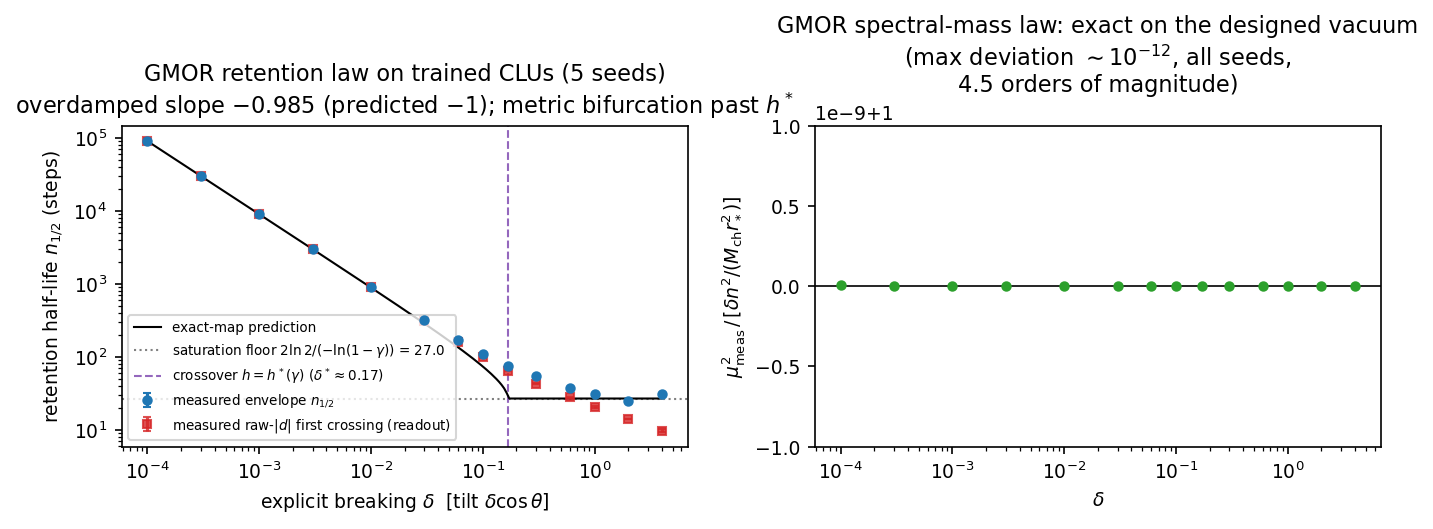
\includegraphics[width=\linewidth]{figs/fig1_gmor.png}
\caption{The curvature-retention relationship, verified on trained checkpoints. Left: The retention half-life $n_{1/2}$ against the analytic tilt $\delta$. The overdamped branch tracks the predicted law at a fitted slope of $-0.985$ (predicted $-1$) before saturating past $h=h^*(\gamma)$ at the curvature-independent floor of $27.03$ steps ($\gamma=0.05$). Envelope half-life (circles) and raw first-crossing time (squares) diverge after the crossover exceptional point. Right: The curvature identity holds flat at $1.000000\pm5\times10^{-12}$ across $4.5$ orders of magnitudes of $\delta$. \emph{Setup: Trained designed checkpoints, analytic tilts, $5$ seeds, dim $4$, $\gamma=0.05$.}(Figure downsized for space constraints, see App.\ref{app:resEx})}
\label{fig:pricelist2}
\end{figure}
\begin{figure}[htbp]\centering
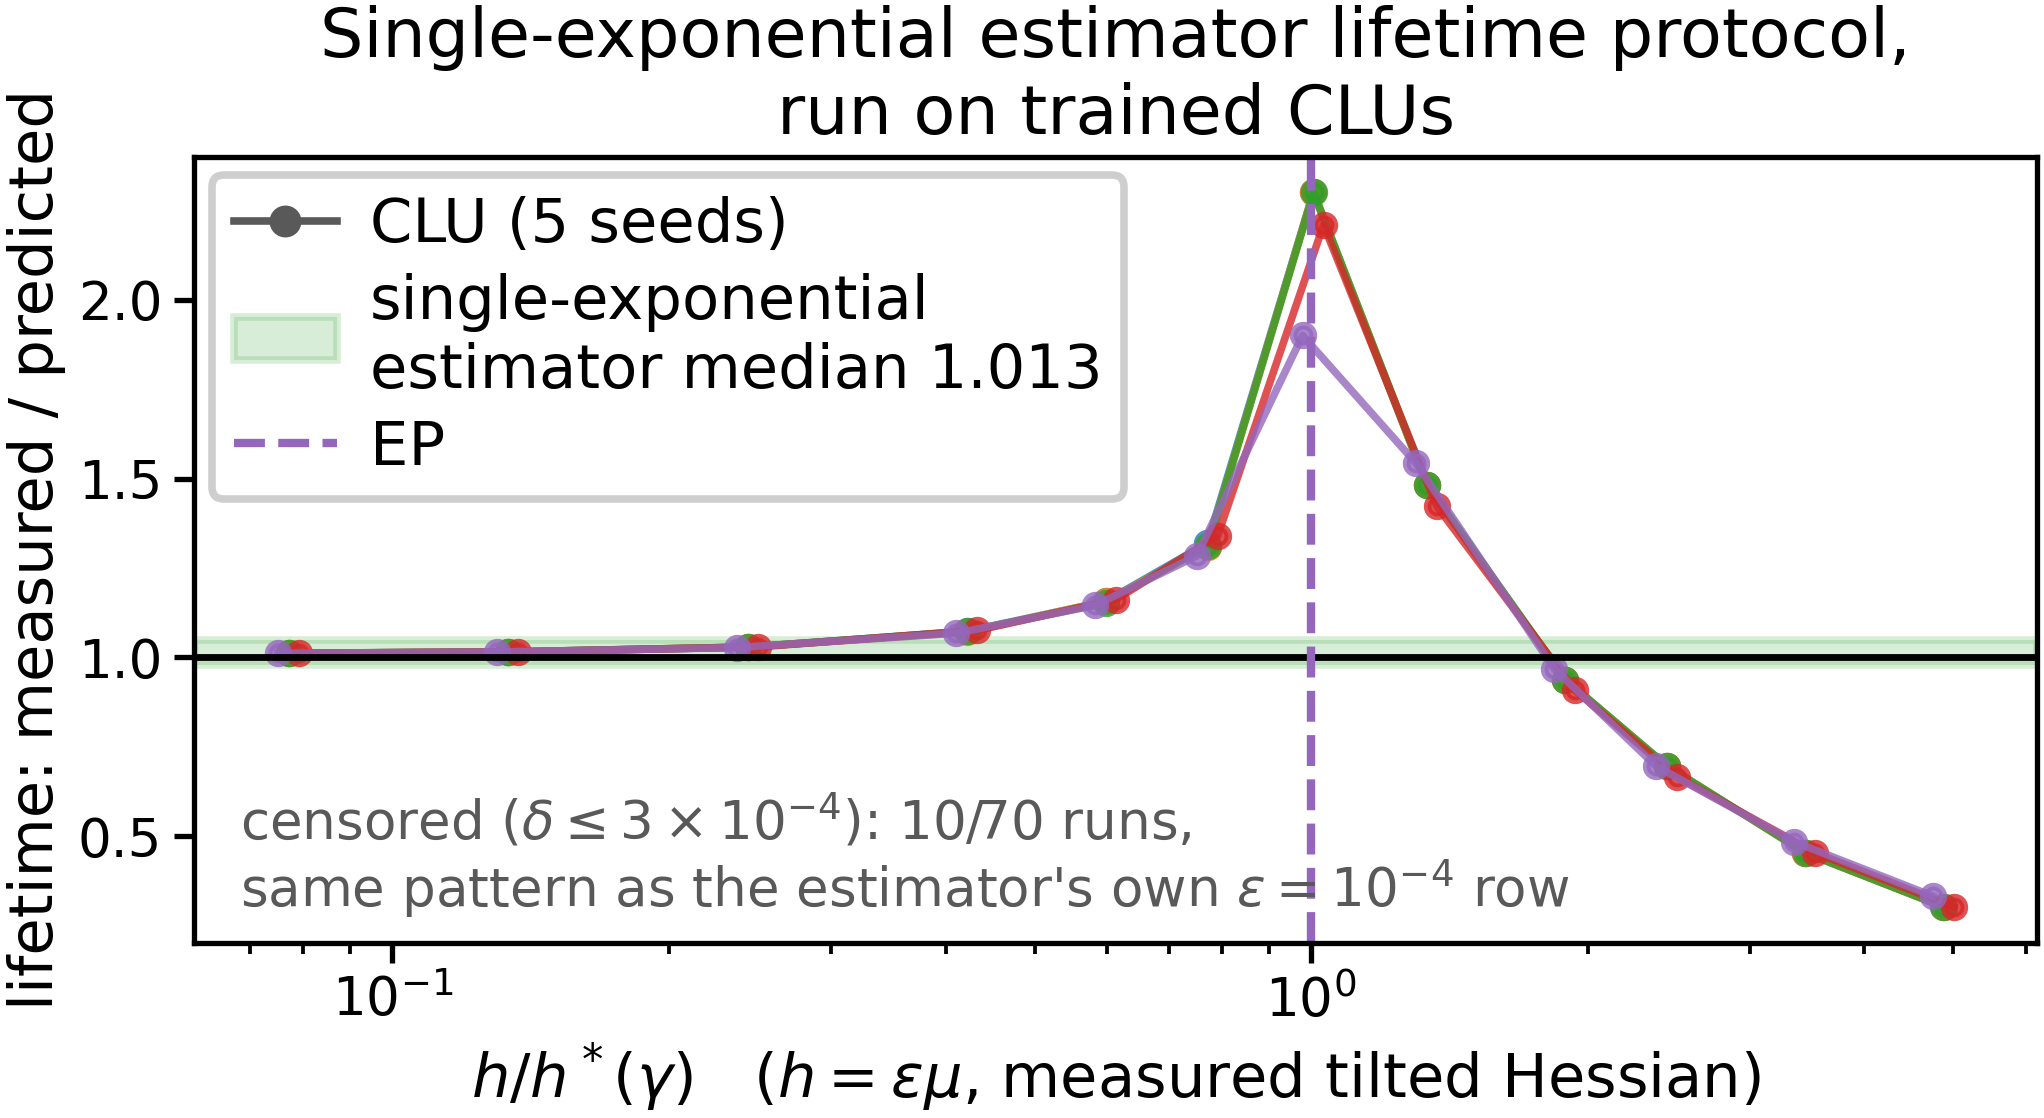
\includegraphics[width=\linewidth]{figs/fig_lifetime_headtohead.png}
\caption{The single-exponential lifetime estimator from~\citet{mo_symmetry-protected_2026}, run unchanged on trained checkpoints, acts as the overdamped face of the CRR. The ratio of measured to predicted lifetime versus breaking magnitude shows containment ($\approx1$) in the overdamped regime. It exhibits a $2.2\times$ delay spike at the exceptional point and degrades to $0.31\times$ underdamped, validating the bounded limits of first-order single-exponential estimation. (Figure downsized for space constraints, see App.\ref{app:resEx})}
\label{fig:lifetime_headtohead2}
\end{figure}

We verify the crossover in Sec.\ref{sec:pricelist} as a genuine exceptional point via two second-order signatures. First, the retention metric bifurcates. Overdamped, the envelope half-life and first-crossing time agree to $0.01\%$; underdamped, they diverge by up to $3.2\times$ at the deepest tilt. Second, the oscillation frequency initiates with a predicted square root dependency. Below $h^*$, the frequency $\varphi=0$ exactly. Above $h^*$, it scales as $\varphi\propto\sqrt{h-h^*}$ with a fitted slope of $0.5165$ (predicted $1/2$). The latch mode natively obeys the transport law $q_\infty=q_0+\varepsilon p_0/(M\gamma)$ to $\le1\%$ across two orders of magnitude of $\gamma$, successfully freezing the written angle to $\le1.2\!\times\!10^{-15}$ rad. These results utilize analytic tilts on trained checkpoints, serving as exact verification of the theory rather than emergent discoveries (further detailed in Appendix~\ref{app:gmor}).

\subsection{Where the CRR does not extend}\label{sec:boundary}

It is often assumed that symmetric training data naturally induces flat geometric directions. \emph{Unlike structural constraints, we find that training data alone does not achieve this on the CLU architecture class.}

A generic MLP potential trained on symmetric data develops softest emergent curvatures of $\mu^2=5.1/5.9/5.4\!\times\!10^{-2}$ across $3$ seeds. Compared to the designed flat mode ($\le2.4\!\times\!10^{-15}$), this presents a gap of $13$-$14$ orders of magnitude. Operationally, this emergent arm functions not on a continuum, but on discrete washboard minima ($\approx1$-$1.6$ bits capacity), where any continuous written coordinate $\delta$ fully relaxes. While the damping-optimum retention law mathematically holds here, the continuous coset register itself is strictly a designed feature, not learned.

\subsection{The CRR survives the training-time correction}\label{sec:cure}

A structural retention advantage is functionally useless if the training objective actively erodes the required potential landscape. \emph{In our system, standard contrastive divergence explicitly destroys the continuous register.}

Wake-sleep contrastive divergence drives the order parameter $r^*$ to zero. At $1000$ epochs, the designed vacuum inverts in $8/8$ runs, eliminating the orbit and generating invariant minimisers with strictly positive $\mu^2$. This represents a manifestation of the fine-tuning problem, where the training objective acts as the primary perturbation. To resolve this, we anchor the condensate using a $V(\text{data})$ energy anchor ($\lambda=100$). Over $5$ seeds, the anchor maintains $r^*=0.911\pm0.016$, trading off weaker noise rejection and a higher wake MSE. \emph{Therefore, we report that the CRR survives this corrective intervention.} Across $3000$ anchored epochs ($\approx20\times$ the baseline erosion horizon), the retention laws remain entirely intact (Appendix~\ref{app:anchor}). The curvature ratio holds to $1.5\!\times\!10^{-12}$, the slope holds at $-0.956$ (the per-point fit over all overdamped rows), the floor remains unchanged, and the exceptional-point onset is bit-identical at $0.5165$.

\section{The laws survive the training-time correction}\label{app:anchor}
See Fig.~\ref{fig:sf3}.
\begin{figure}[htbp]\centering
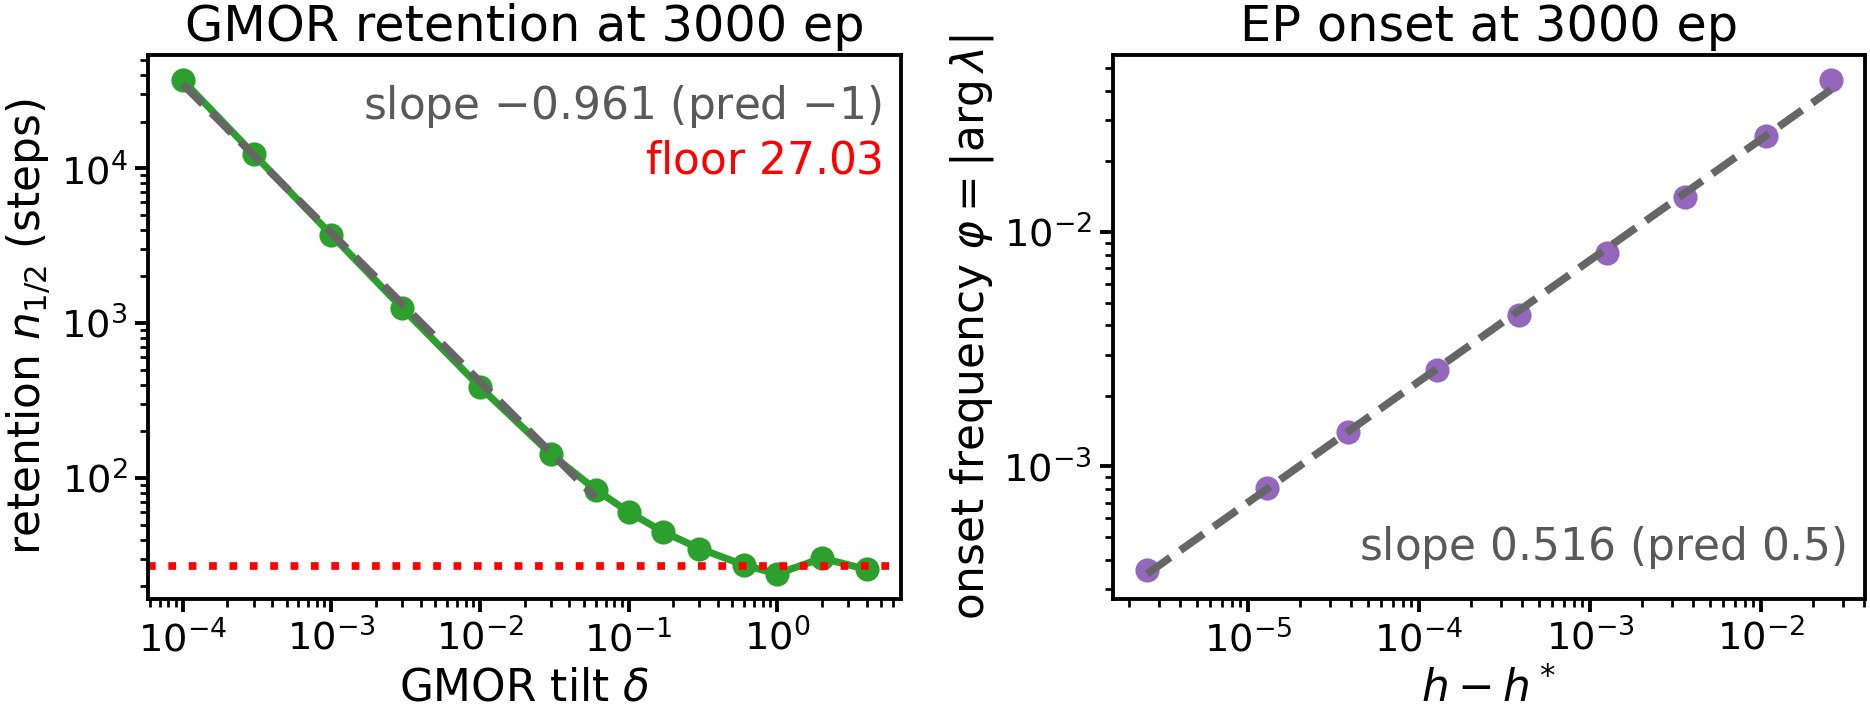
\includegraphics[width=\linewidth]{figs/fig2_anchor_cure_laws.png}
\caption{The CRR laws survive the applied anchor correction at $3000$ epochs ($\approx20\times$ the erosion horizon; anchored $\lambda=100$, $3$ seeds). Left: The retention law $n_{1/2}$ versus tilt $\delta$ demonstrates anchored points tracking the predicted slope (fitted $-0.961$ against predicted $-1$; the seed-mean OLS over the $7$ overdamped $\delta$) before saturating at the curvature-independent floor of $27.03$. The $\mu^2/\delta$ ratio maintains $1.0000\pm10^{-12}$ stability over $4.6$ orders of magnitude. Right: The exceptional-point onset follows $\varphi\propto\sqrt{h-h^*}$ above the critical threshold, with a fitted slope of $0.516$ (predicted $0.5$) and exactly $\varphi=0$ below, remaining bit-identical to the baseline $150$-epoch measurement. \emph{Results map to a designed testbed under the applied cure, providing structural evidence that the recipe maintains integrity through erosive training scales.}}
\label{fig:sf3}
\end{figure}

\section{The explicit trade-off of the physical prior}\label{app:loan}

We explicitly clarify that this section analyzes the baseline cost of embedding physics priors and does not serve as a primary performance claim.

Evaluating the system against parameter-matched controls (dimension $4$, $150$ epochs, $3$ seeds, identical MLP potential) reveals a strict Pareto tradeoff. Conserving phase-space volume inherently provides bounded (BIBO) dynamics inside the coercive-potential scope ($1.00$ versus $0.33$ for the broken-volume baseline), protects a near-flat direction ($\mu^2=0.008$ versus $0.122$), and enables vacuum survival under contrastive-divergence training ($r^*=0.72$ versus $0$). \emph{However}, this strict prior fundamentally constrains raw fitness. An unconstrained twin achieves an evaluation MSE of $0.0128$, outperforming the constrained unit's $0.190$. This penalty is proven mathematically to be contraction-forbidden by the volume conservation axiom, as the broken-volume baseline precisely recovers $\approx2.4\times$ of the performance gap purely by leaking volume.

The constrained model's primary asset is bounded execution by construction, not achieving the lowest steady-state MSE. While the twin model's raw fit diverges dramatically after $\approx700$ steps (reaching an MSE of $196$ at $5000$ steps), the physically-informed unit maintains a bounded plateau of $\approx0.20$--$0.23$. Only global damping mechanisms recover the lost fit; introducing a learned friction field does not functionally substitute.

\emph{Data configuration: Dimension $4$, hidden $64$, learned-Newtonian kinetic term, $\mathrm{dt}=0.05$, circle $R=1\times256$, $150$ epochs, $3$ seeds, wake-only objective except the $\gamma_\phi$ rung. Cumulative fit MSE against horizon is measured on the stationary circle-vacuum orbit, parameter-matched to $\pm0.2\%$ (CLU $4549$ / broken-volume $4557$ / twin $4551$).}

\begin{center}
\begin{tabular}{lcccc}
\toprule
Horizon (steps) & \textbf{Twin} & \textbf{CLU} & Broken-Volume & LSTM \\
\midrule
$10$ & $\mathbf{2.9{\times}10^{-6}}$ & $2.2{\times}10^{-5}$ & $1.1{\times}10^{-4}$ & $7.5{\times}10^{-2}$ \\
$50$ & $\mathbf{6.2{\times}10^{-5}}$ & $1.2{\times}10^{-3}$ & $1.0{\times}10^{-3}$ & $4.9{\times}10^{-2}$ \\
$100$ & $\mathbf{2.4{\times}10^{-4}}$ & $1.2{\times}10^{-2}$ & $4.1{\times}10^{-3}$ & $4.9{\times}10^{-2}$ \\
$500$ & $\mathbf{1.1{\times}10^{-2}}$ & $1.8{\times}10^{-1}$ & $9.7{\times}10^{-2}$ & $7.7{\times}10^{-2}$ \\
$1000$ & $3.2{\times}10^{-1}$ & $\mathbf{2.0{\times}10^{-1}}$ & $1.2{\times}10^{-1}$ & $9.9{\times}10^{-2}$ \\
$5000$ & $1.96{\times}10^{2}$ & $2.2{\times}10^{-1}$ & $\mathbf{1.4{\times}10^{-1}}$ & $1.3{\times}10^{-1}$ \\
\bottomrule
\end{tabular}
\end{center}

\emph{We emphasize that the following table represents an independent wake-only experiment. The absolute MSE scale and its associated twin ($0.0047$) are not mathematically cross-comparable with the prior parameter-matched table (twin $0.0128$) due to variations in seeds and training objectives. Comparisons must remain restricted to intra-table relative ratios.}

\begin{center}
\begin{tabular}{lccccc}
\toprule
Model Variant & Eval MSE & \% Gap Recovered & BIBO & Latch Drift & Flat $\mu^2$ \\
\midrule
Twin (No Physics) & $0.0047$ & $100\%$ (Ref) & $1.00$ & --- & --- \\
CLU Conservative ($\gamma=0$) & $0.2066$ & $0\%$ (Ref) & $1.00$ & $0.778$ & $5.2{\times}10^{-3}$ \\
$+\gamma$ Global ($\gamma=0.05$) & $0.0216$ & $\mathbf{92\%}$ & $1.00$ & $0.778$ & $5.2{\times}10^{-3}$ \\
$+\gamma_\phi$ Learned Field ($K=2$) & $0.2548$ & $-24\%$ & $1.00$ & $0.706$ & $2.1{\times}10^{-2}$ \\
\bottomrule
\end{tabular}
\end{center}

\section{The autonomous-retention head-to-head against learned baselines}\label{app:retention}

Figure~\ref{fig:retention} reports the autonomous-retention protocol run against the learned baselines.

\begin{figure}[htbp]\centering
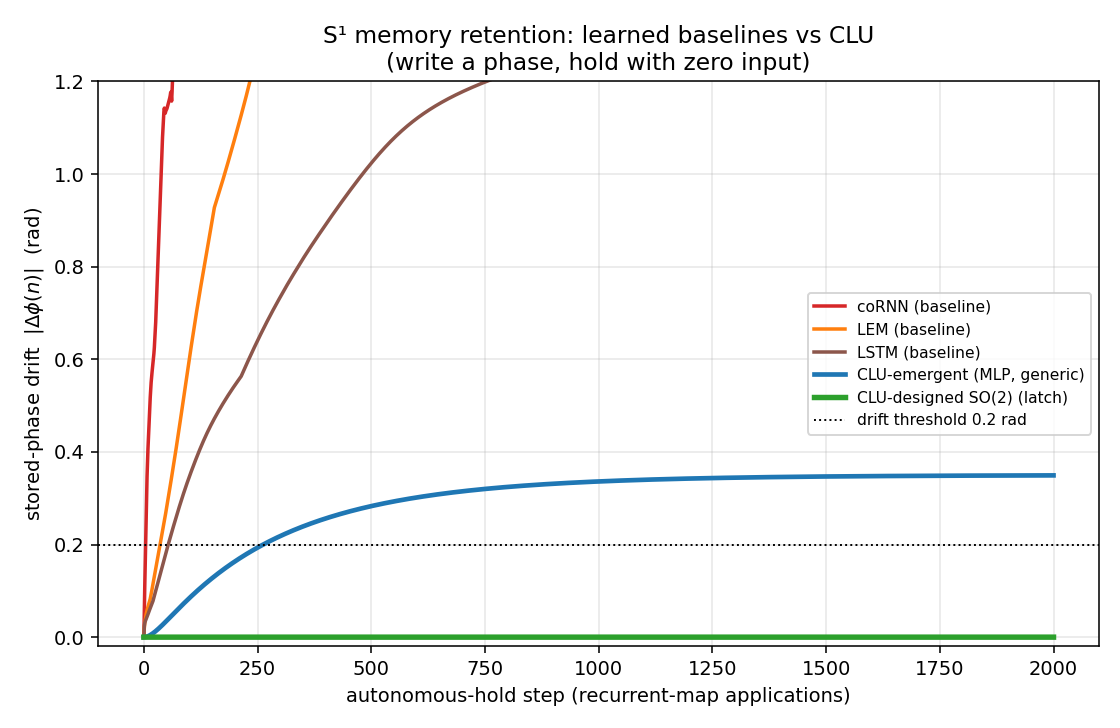
\includegraphics[width=\linewidth]{figs/fig3_retention_overlay.png}
\caption{Autonomous retention evaluated via the $S^1$ protocol (arXiv:2605.03338). A designated phase is encoded, the input is systematically removed, and structural drift of the stored phase is tracked continuously across unspooled map applications. The learned baselines exhibit critical phase loss within $\approx5.6/56/69$ map-steps (coRNN/LEM/LSTM) as the latent coordinate completely randomizes beyond $1.2$ rad. In contrast, the generically-trained symplectic unit maintains a bounded state of $\approx0.35$ rad, and the symmetry-designed unit registers strictly zero drift. Baseline and emergent measurements represent the median across $5$ and $3$ seeds respectively, while the designed curve is a single representative checkpoint. Experimental constraints: Dimension $4$, hidden $64$, single-core CPU execution, drift threshold defined at $0.2$ rad, evaluated at deterministic $T=0$.}
\label{fig:retention}
\end{figure}

\section{Per-step compute requirements}\label{app:compute}

\paragraph{Honest compute gap:} We emphasize that the raw $263$-to-$69$ map-step advantage presented in the comparisons against LSTMs, LEMs and CoRNNs is not a normalized compute analysis. A single unoptimized Verlet update costs $\approx6.2\times$ the wall time of an LSTM cell and $\approx3.1\times$ that of a LEM cell ($\approx14$-$15\times$ FLOPs). When normalized per unit of retention, our architecture demands significantly more computational overhead. However, the CLU is a nascent idea and compute optimization is deferred to future work.

We document the explicit performance normalization factoring that necessitates our retirement of the naive ``map-step'' claim as a formal metric of compute efficiency. Measured strictly on a single-core CPU via f32 XLA, one CLU dissipative-Verlet step entails two $\nabla_qV$ backpropagations through a $\dim 4\to64\to64\to1$ tanh MLP with a learned-Newtonian kinetic term. Wall time is the median of $7$ scan-amortized repetitions over $2{\times}10^5$ steps; the na\"ive single-call timing is dispatch-bound at a $\approx5\,\mu$s floor and is \emph{not} reported.

\begin{center}
\begin{tabular}{lccc}
\toprule
Unit Configuration & Parameters & FLOPs/Step & Wall ns/step \\
\midrule
Unoptimized CLU Verlet (h$64$, dim $4$, KDK) & $4549$ & $\mathbf{36148}$ & $1554$ \\
LSTM cell (h$16$) & $1186$ & $2512$ & $252$ \\
LEM cell (h$16$) & $1186$ & $2400$ & $500$ \\
\bottomrule
\end{tabular}
\end{center}

\begin{center}
\begin{tabular}{lcc}
\toprule
Normalization Standard & CLU vs.\ LSTM & CLU vs.\ LEM \\
\midrule
Raw map-steps ($263$ vs.\ $69$/$56$) & $3.8\times$ longer & $4.7\times$ longer \\
FLOP-normalized & $\mathbf{54.8\times}$ more & $\mathbf{70.7\times}$ more \\
Wall-normalized & $\mathbf{23.5\times}$ more & $\mathbf{14.6\times}$ more \\
\bottomrule
\end{tabular}
\end{center}

\textbf{Confound:} the comparison is not width-matched, CLU at hidden $64$ with two gradient evaluations against baselines at hidden $16$; a width-matched CLU would narrow the gap, but the sign is still robust because the Verlet step requires two potential backpropagations, and the $263/69/56$ retention numbers come from these specific configurations. The measurement is single-core CPU at batch $1$; GPU or batched throughput could shift the wall ratios, though not the FLOPs.

\section{Documented negative results and formal limitations}\label{app:neg}

The limitations of this early-stage works are broadly:

\begin{itemize}
    \item \textbf{Operational Scope:} Measurements rely on a laptop CPU, latent dimension $4$ and the $S^1$ testbed.
    \item \textbf{Analytical Limits:} The solvable core is quadratic. Trained measurements remain localized to the critical points of $V_\theta$. Finite-$T$ diffusion laws are exclusively bounded by fluctuation-dissipation theorem constraints.
    \item \textbf{Task Benchmarking:} We do not present or claim external task benchmark superiority since this is deferred to future work.
    \item \textbf{Off-Distribution Stability:} BIBO stability bounds apply only to the autonomous, designed setting. We make no claims regarding input-driven off-distribution stability on trained networks.
    \item \textbf{Substrate Scope:} These laws govern a latent memory register; end-to-end performance additionally depends on the encoder, measured separately, with its parameter and state-byte budget ledgered.
\end{itemize}

This appendix is tree-level and classical: no loops, chiral logarithms, running low-energy constants or anomalies. It is probe-only on already-trained checkpoints, with the spurion off by default so as to be bit-compatible with every result elsewhere, on one architecture family: designed exact $SO(2)$, dimension $4$, laptop CPU. The emergent MLP arm is untested and would carry its own self-breaking $\delta_{\rm eff}$, so GMOR there should be tested as $\delta\to\delta+\delta_{\rm eff}$.

We also structurally record all hypothesis failures and architectural limitations evaluated during this work.

\begin{center}
\begin{tabular}{@{}p{1.52in} p{1.52in} p{2.06in}@{}}
\toprule
Tested Hypothesis & Operational Result & Supporting Measurement \\
\midrule
Does a learned inertial mass isotropize strictly on symmetric data? &
No, the breaking is fundamentally invisible to the standard Hessian and the latch, appearing only as bounded Noether-charge oscillations. &
Log-mass split ratios are $0.98$ / $1.18$ / $5.4$ from init to $150$ ep; charge amplitudes $5.4/1.6/0.082{\times}10^{-2}$; tied controls exactly $1.0000$. \\[2pt]
Does wake-sleep contrastive divergence preserve designed degenerate vacua? &
No, it strictly inverts it. A $V(\text{data})$ energy anchor must be introduced to stabilize it. &
$r^*\to0$ across $8/8$ iterations at $1000$ ep; inversion at epoch $116$/$442$/$959$ by sleep frequency; anchor $\lambda{=}100$ successfully holds $5/5$ seeds at $r^*{=}0.911\pm0.016$. \\[2pt]
Does an emergent (MLP) unit maintain a continuous coset register? &
No, the continuous framework is strictly designed. Emergent variations resolve to discrete washboard minima configurations. &
$1-|\lambda_{\rm coset}|\approx10^{-3}$ against the designed $\le1.1{\times}10^{-15}$, $\sim\!12$ orders; written $\delta$ retained $\le2.1{\times}10^{-3}$; capacity $\approx1$--$1.6$ bits. \\[2pt]
Can explicit-breaking coefficients function as reliable lifetime dials on learned stores? &
No, increasing the breaking magnitude inversely lowers the softest eigenvalue, and absolute coercivity dictates the ceiling limit. &
$\lambda_{\min}$ ranges $+0.0994\to-8.2846$ and $+0.3291\to-1.1980$ over four orders of magnitude of breaking; hard operational ceiling observed at $\tau_{\max}=\Gamma/2\alpha=4.0$; tilt-vacuum residual $0.140$--$0.343$ against a random-direction baseline $1/\mathrm{dim}=0.167$. \\[2pt]
Is the coded momentum-coupled Langevin sampler FDT-exact across all kinetic modes? &
No, it proves FDT-exact strictly in Newtonian execution. Under relativistic operations, no noise scale converges the chain to a Gibbs invariant. &
Required per-mode scale verified as $\sigma^\star_i=\sqrt{M_iT\gamma(2-\gamma)}$. \\[2pt]
\bottomrule
\end{tabular}
\end{center}

\begin{center}
\begin{tabular}{@{}p{1.52in} p{1.52in} p{2.06in}@{}}
\toprule
Tested Hypothesis & Operational Result & Supporting Measurement \\
\midrule
Do raw $n_{1/2}$ exponents discriminate designed from emergent stores? &
No, a matched designed control on the same grid gives the same slopes, both carrying the $\ell_\theta/\Delta$ boundary layer. No $n_{1/2}$ may be quoted without its $\Delta$ and $\ell_\theta/\Delta$. &
Designed control $\mathrm{d}\log n_{1/2}/\mathrm{d}\log T=-0.53,-0.60,-1.04$ and $\mathrm{d}\log n_{1/2}/\mathrm{d}\log\gamma=+0.78,+0.63,+0.55$; $\ell_\theta/\Delta$ up to $2.0$. \\[2pt]
Do a learned friction field and a curvature governor compose usefully? &
No, the pair is Pareto-dominated by either alone, and a learned compact-support gate under-covers without accurate placement. &
Locus discovery $2/6$ before adaptive-$K$, $2/3$ after; best learned rejection $0.861$; a $\lambda$ re-sweep does not approach the oracle. \\[2pt]
Can friction stabilize a saddle, or an energy gate catch isoenergetic escape? &
No, only curvature control of $V_\theta$ and the mass-anisotropic cap $v_i^{\max}=c/\sqrt{M_i}$ bound expanding or isoenergetic modes. &
$\lambda_+>1$ for all $\gamma$, with $\min_\gamma(\lambda_+-1)=1.4{\times}10^{-5}$. \\[2pt]
Is a mean-spectrum chaos regularizer informative? &
No, it is degenerate; a chaos penalty must use a max or positive-part statistic. &
--- \\[2pt]
\bottomrule
\end{tabular}
\end{center}

\emph{We clarify specific architectural limitations identified in these negatives:} The closed-form charge-oscillation amplitude bounds strictly dictate on-vacuum-orbit behaviors. Consequently, anisotropic channels continue to latch with mathematically infinite half-lives; mass-tying serves primarily to enforce angle-independent write currents rather than structurally save the register itself. Furthermore, we explicitly emphasize that explicit breaking parameters do not scale linearly with system retention outside of purely designed $SO(2)$ geometric environments.

\section{Contextualizing prior work boundaries}\label{app:pos}

To ensure precise attribution and clearly demarcate the novelty of our contributions, we explicitly contextualize our methods against closely associated literature:

\begin{enumerate}
    \item \textbf{Retention Guarantees in State-Space Models:} Architectures such as HiPPO-LegS~\citep{gu_hippo_2020} maintain $O(tL/\sqrt N)$ retention guarantees, utilizing exact timescale equivariance devoid of discrete tuning boundaries. We do not assert that our $\mu^2$-driven continuous curvature spectra out-perform these bounds natively.
    \item \textbf{Retrieval as Rollout:} Treating continuous retrieval sequences as deterministic dynamical rollouts is fully established by \citet{kong_reservoir-computing_2024}. Our implementation builds on this by enforcing strict symplecticity and Hamiltonian constraints.
    \item \textbf{Continuity as a Novelty:} The foundational mechanics of continuous and soft-memory mapping are native to the Neural Turing Machine~\citep{graves_neural_2014} and DNC lineages. Key/value entanglement phenomena diagnosed in these models~\citep{csords_improving_2019} technically map onto our architecture, though our evaluation focuses strictly on geometric state drift.
    \item \textbf{Transformer Scaling Comparisons:} The frameworks explored in this paper are analytically bounded tools ($1$-$1.6$ bits per emergent register). We make no claims regarding benchmark scaling or general superiority against current Transformer implementations.
\end{enumerate}

\section{GMOR verification on trained checkpoints}\label{app:gmor}

\emph{Data configuration: Designed testbed mapped with analytic tilts and an analytic spurion to verify the theory's exactness. Evaluated on $5$ primary seeds at $150$ epochs and $3$ anchored seeds at $3000$ epochs, dimension $4$, executed on CPU with $f64$ probes and zero network retraining. GMOR-proper results below, are a supporting result, not one of this paper's claims.}

\subsection{The foundational retention scaling law} The retention scaling law $n_{1/2}\propto\mu^{-2}$ functions analytically as a Gell-Mann--Oakes--Renner (GMOR) relationship~\citep{gell-mann_behavior_1968} within the spectral mass context ($\mu^2F^2=\delta\Sigma$). Over $70$ distinct tilt rows mapped across a machine-flat trained vacuum, the constitutive identity aligns to $3.2{\times}10^{-10}$. Across $4.5$ orders of magnitude, the scaling curvature ratio holds to $1.000000\pm5{\times}10^{-12}$. The $\sqrt{h-h^*}$ onset holds down to $h-h^*=2.6{\times}10^{-6}$ on a fine multiplicative grid ($h-h^*\in[-4.2{\times}10^{-3},2.6{\times}10^{-2}]$). Where the quality factor permits ($f=2,4$), the trajectory frequency matches the Jacobian frequency to $0.06$--$0.3\%$; near onset the mode decays before one period completes, so the exceptional point is spectroscopically real but dynamically silent there.

\subsection{Secondary bounds of the damping corollary} Modulating the damping constant $\gamma$ at a fixed spectral mass yields a distinctly non-monotone retention profile. The function $n_{1/2}(\gamma)$ forms a V-shaped curve, identifying its minimum directly beneath the exact critical-damping value $\gamma^*\approx2\varepsilon\mu$. Consequently, an isolated evaluation of retention scaling at a single $\gamma$ remains technically uninformative regarding the functional sign of $\partial n_{1/2}/\partial\gamma$ unless its position relative to the damping critical threshold is analytically specified.

\subsection{Ambient spurion integration} To disentangle the radial dependence masked by simple angular tilts ($V\to V+\delta(1-\cos n\theta)$), we introduce a linear ambient spurion ($V\to V-\delta\,(u\cdot q)$). Under this condition, the vacuum radius dynamically tracks with $\delta$, allowing explicit and separate verification of the pseudo-Goldstone spectral mass ($\mu^2$), the decay constant ($F^2$), and the condensate ($\Sigma$). Across $8$ trained checkpoints mapped from $\delta\in[10^{-8},0.3]$, the absolute deviation between $\mu^2F^2$ and $\delta\Sigma$ is structurally bounded by $\max|\mu^2F^2-\delta\Sigma|=1.33{\times}10^{-15}$.

\subsection{Condensate tracking} Evaluated via geometric parameterizations, Hellmann-Feynman theorem proofs, and finite difference differentials, the running condensate $\Sigma$ scales by $+16.1\%$ to $+210.1\%$ across the full evaluated $\delta$ grid, operating entirely blind to the natively shipped angular tilt functions.

\begin{figure}[htbp]\centering
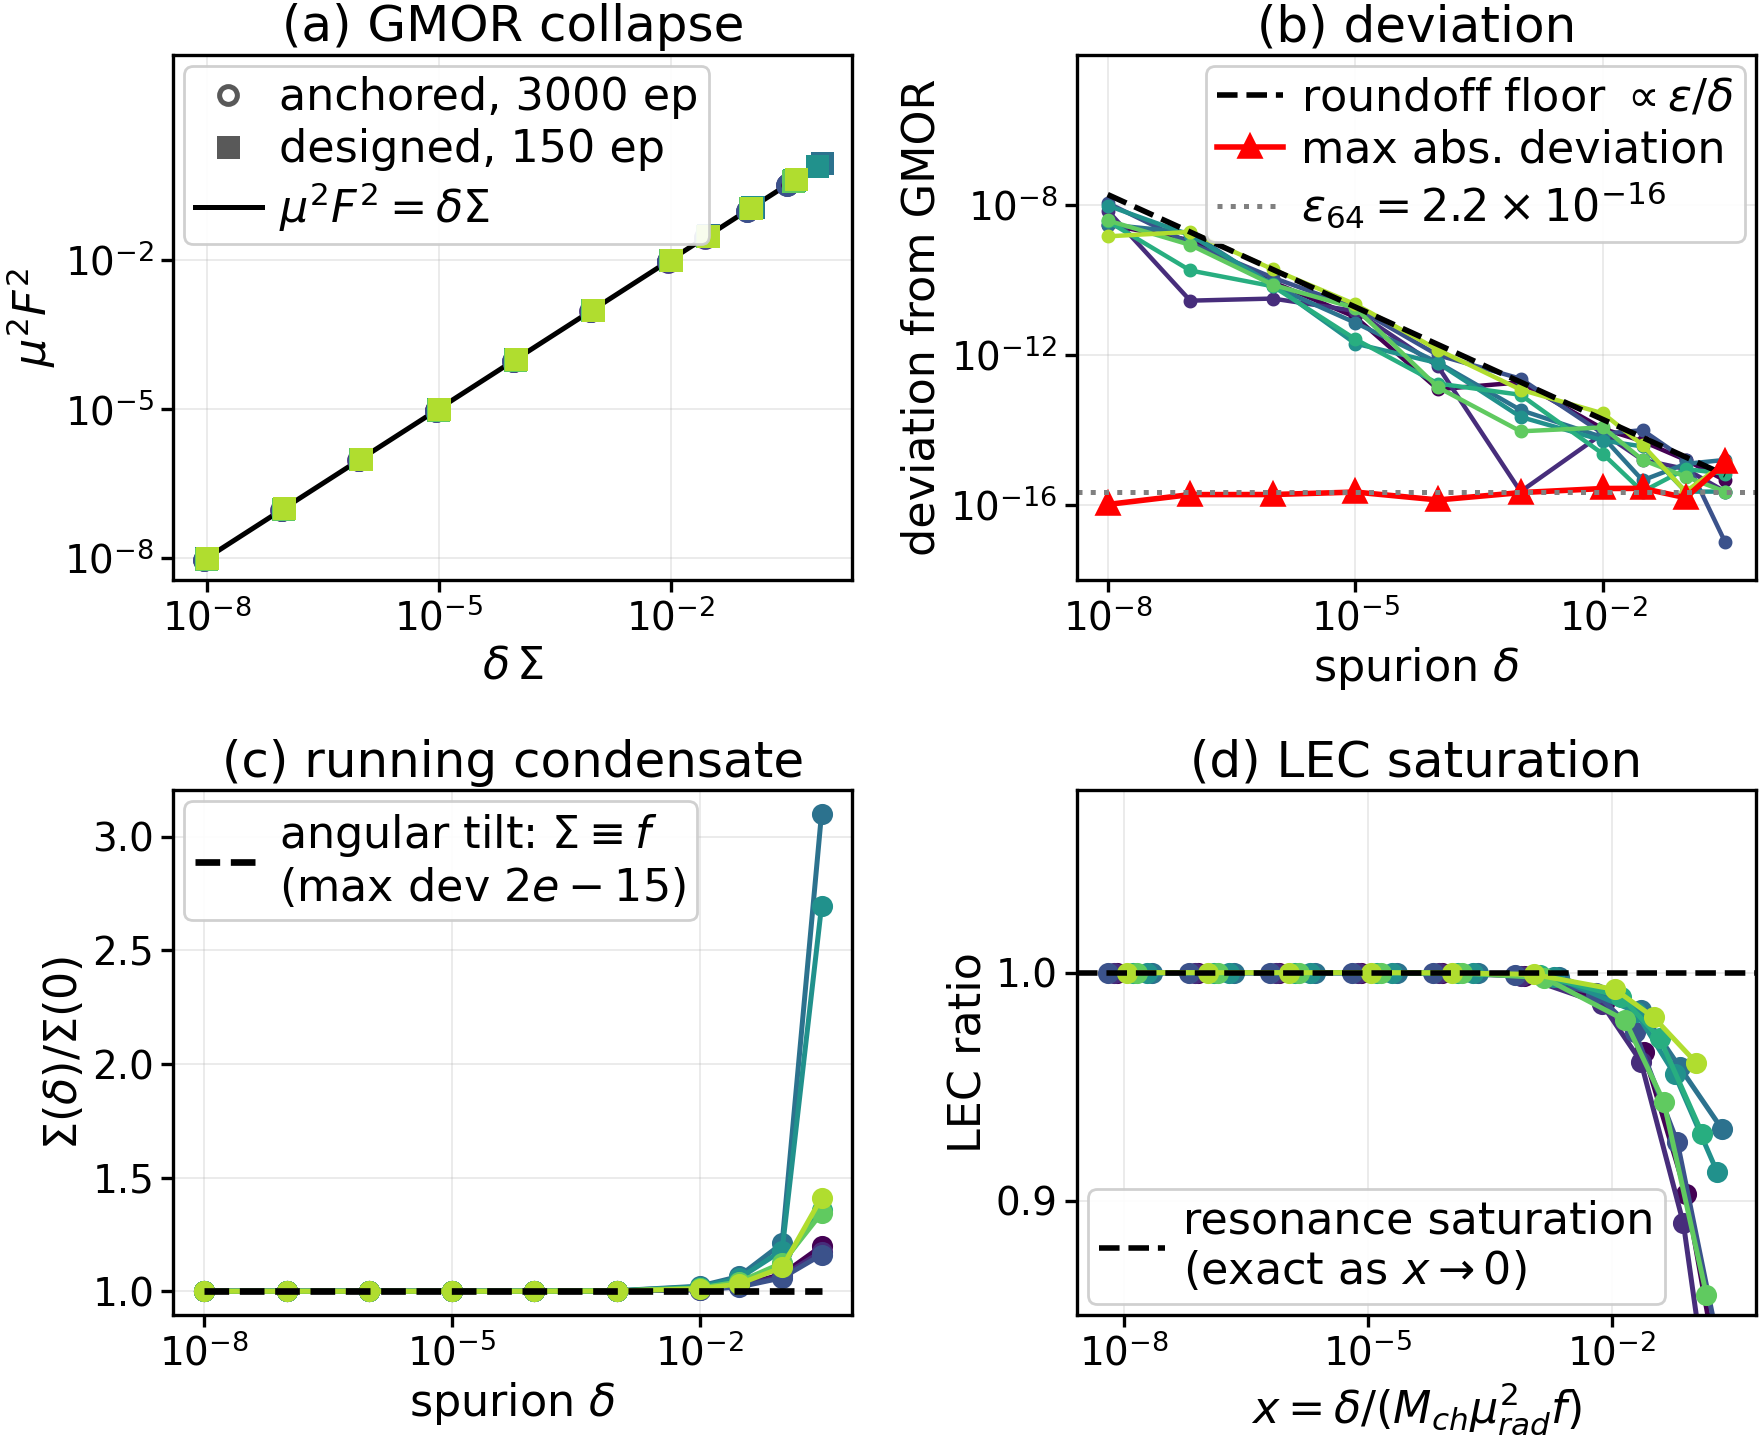
\includegraphics[width=\linewidth]{figs/fig3_gmor_condensate.png}
\caption{Full GMOR structural verification measured via a linear ambient spurion. (a) Total collapse of $\mu^2F^2=\delta\Sigma$ mapped precisely across $8$ orders of magnitude of $\delta$ tracking. (b) Bound absolute deviations pinned at the exact $f64$ limits ($\le1.33{\times}10^{-15}$) juxtaposed against autodiff relative-roundoff thresholds. (c) The functional running condensate $\Sigma(\delta)/\Sigma(0)$ scaled against an angular tilt baseline. (d) The asymptotic alignment of the low-energy-constant ratio as the chiral expansion variable $x$ scales toward zero.}
\label{fig:gmor}
\end{figure}

GMOR holds to machine precision in absolute terms at every $\delta$; relative exactness ($\le2.7{\times}10^{-14}$) is demonstrated for $\delta\ge10^{-2}$. The growing \emph{relative} deviation at small $\delta$ is not a failure of the law but the roundoff floor of the autodiff Hessian: the angular curvature is $K_{\theta\theta}=\delta/r^*$, reconstructed as a difference of $O(\lVert K\rVert)$ terms, so its absolute error is $\sim\epsilon\lVert K\rVert$ and its relative error $\sim\epsilon/\delta$. This was confirmed directly: on the analytic Mexican hat a cancellation-free Hessian returns relative deviation $1.1$--$2.2{\times}10^{-16}$ at \emph{every} $\delta\in[10^{-8},0.3]$, while the autodiff Hessian on the same potential returns $2.28{\times}10^{-8}\to4.22{\times}10^{-15}$ across that range, exactly $\propto1/\delta$. The same $\epsilon/\delta$ floor applies to every $\mu^2$ probe in this paper; all other sweeps here use $\delta\ge10^{-4}$, where the floor is $\sim10^{-12}$ and the quoted relative agreements are sound.

\subsection{The expansion variable, and where it stops being small.} With $\mu^2_{\rm LO}\equiv\delta\Sigma(0)/F^2(0)$, the theory predicts a \emph{relative} leading-order error $x\equiv\delta/(M_{\rm ch}\mu_{\rm rad}^2f)$; this is the $x$ of Figure~\ref{fig:gmor}(d).

\section{Extended discussion and future directions}
\label{app:exDisc}

The natural generalization of the present $SO(2)\to\{e\}$ register is a breaking pattern $G\to H$ whose memory manifold is the coset space $G/H$; by the same tree-level argument as App.~\ref{app:curcos}, its $\dim(G/H)$ orbit tangents are exactly flat. The choice of stabilizer would then select which components of the stored latent state are retained. On designed geometries of this class, a controlled breaking that lifts only a subset of those directions would yield a mixed spectrum of exact Goldstone latches and pseudo-Goldstone registers of finite, curvature-set lifetime. This is a direction on which this paper offers no evidence, but is part of our future work.

The broader motivation is a learning regime in which such symmetries, and their controlled breaking, arise emergently rather than by construction; the negative of Sec.~\ref{sec:boundary} shows the present recipe does not produce this, and closing that gap guides the directions above.

\end{document}
